\label{chapter:correlatos}

\par
\textcolor{red}{Neste capítulo serão apresentados alguns trabalhos relacionados que envolvem mineração de dados...} 

\section{Mineração de Dados Educacionais nos Resultados do ENEM de 2015}

\par
O trabalho de \citeonline{Simon2017} tem como objetivo em gerar um modelo preditivo da base de desempenho médio na área de ciências da natureza e suas tecnologias dos alunos de escolas do ensino médio, baseado nos dados públicos obtidos do Exame Nacional do Ensino Médio (ENEM) de 2015. Tal motivação foi pelo fato do cenário preocupante do baixo desempenho dos alunos do ensino básico no Brasil, conforme os dados de 2015 do PISA (\textit{Programme for International Students Assessment}).

\par
Segundo \citeonline{Simon2017} foi feito o pré-processamento dos dados do ENEM fornecidos pelo INEP, sendo que para cada área avaliada apresentavam-se 25 colunas que representavam uma informação ou variável, onde cada uma delas eram divididas em três categorias: características da escola, indicadores e desempenho. Das 25 variáveis, apenas 9 foram selecionadas como importante para a mineração de dados conforme o indicador da coluna Id representado na Figura 11. 

\begin{figure}[!htp]
	\begin{center}
    \caption{\label{fig:waveform_fig} Variáveis disponibilizadas pelo ENEM por escola.}
	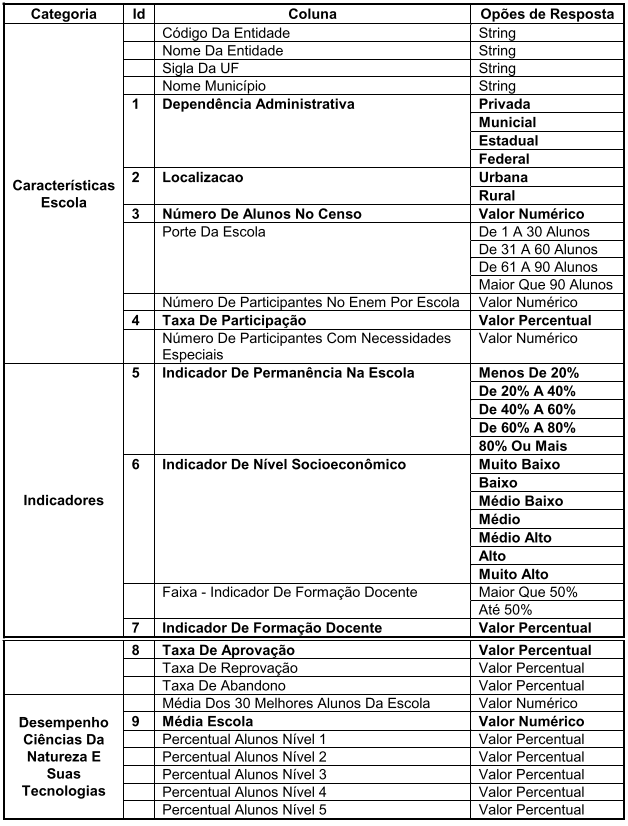
\includegraphics[scale=0.99]{Figuras/Tabela_ENEM.png}
	\end{center}
    \legend{Fonte:\cite{Simon2017}}
\end{figure}

\par
\citeonline{Simon2017} destacaram que a variável Média Escola indicava o desempenho médio dos alunos da escola na área de ciências da natureza e suas tecnologias, onde esses dados eram fornecidos como valor numérico pelo INEP, então para facilitar a mineração dos dados, ele teve que converte-lo para uma categoria mais limitada que foi dividida em quatro valores possíveis, segundo a escala prevista pelo INEP conforme a Figura 12. Os dados fornecido pelo INEP, vinham em uma planilha no formato .xlsx e teve que ser convertido para .csv, pois, o formato não era suportado pelo software WEKA.


\begin{figure}[!htp]
	\begin{center}
    \caption{\label{fig:waveform_fig} Categoria para os valores Média Escola.}
	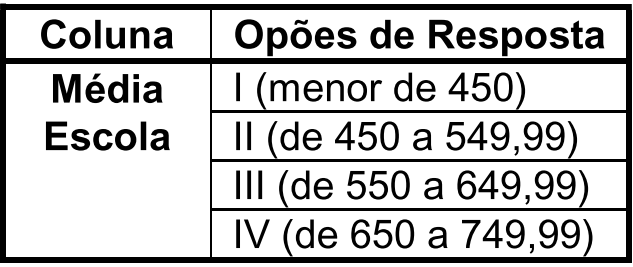
\includegraphics[scale=0.50]{Figuras/Tabela_ENEM_2.png}
	\end{center}
    \legend{Fonte:\cite{Simon2017}}
\end{figure}

\par
Relacionando os fatores socioeconômicos e o índice de desempenho médio em ciências da natureza e sua tecnologias dos alunos, \citeonline{Simon2017} construiu um modelo preditivo utilizando a técnica de mineração de árvore de decisão. Tal técnica, usou o algoritmo j48 através do software WEKA, que foi executado utilizando a opção de \textit{cross-validation}, onde o valor para \textit{fold} era igual a 10 e com a variável depedente Média Escola. Com a árvore obtida, demonstrou como variável independente mais relevante foi a variável Tipo Escola, que se divide entre quatro valores: privada, federal, estadual e municipal.

%Variavel dependete seria o resultado e a variavel independente seria o caminho que ele iria percorre até o resultado. Exemplo: variavel dependete (aluno passou | aluno não passou), variavél independente(entregou os trabalhos, participou das aulas, tirou nota boa na prova, numeros de faltas e etc).

\par
Depois da variável Tipo Escola, a variável hierarquicamente seguinte é a Nível socioeconômico e a partir dela as váriaveis seguintes se alternam de posição conforme as funções dos valores dos níveis superiores. Como resultado, sobre o desempenho médio dos alunos na área de ciências da natureza e suas tecnologias, as categorias que mais se destacaram foram a III e IV, acima de 550 pontos, que ocorreram nas escolas: privadas e estaduais com o nível socioeconômico muito alto, federais com o nível médio alto e muito alto e municipal com o nível médio alto.

\par
\textcolor{red}{Há alguns pontos deste trabalho que se relacionam ao trabalho que pretendo fazer, uma delas é a base de dados dos fatores socioeconômico e outras informações fornecidos do ENEM pelo INEP, que esta relacionado na parte de pré-processamento, é semelhante aos dados fonecidos pela Comissão Permanente do Vestibular (CPV) da UFRR, como base eu poderia pegar as mesmas variáveis que foram escolhidas no trabalho de \citeonline{Simon2017} para agilizar o meu trabalho de minerar os dados mais imporntante para solucionar o meu problema.}
\par
\textcolor{red}{Outro ponto importante é o modelo preditivo que ele abordou, que é a técnica de mineração de árvore de decisão que utiliza o algoritmo J48 do software WEKA, já que eu utilizarei a mesmo conceito de modelo, poderia utilizar a opção de \textit{cross-validation}, no caso o K-\textit{folds}, que ele usou para os treinos e testes dos dados para a validação do modelo.}



\section{Prática de Mineração de Dados no Exame Nacional do Ensino Médio}

\par
O trabalho de \citeonline{Silva2014}, apresenta um estudo de mineração de dados educacionais, mais especificamente, utilizando a tarefa de Associação de Dados de MD no intuito de encontrar padrões de regras nos dados dos questionários socioeconômicos e resultados das provas do Exame Nacional de Ensino Médio (ENEM), fornecidos pelo INEP. O objetivo é de executar as etapas do KDD para o processamento dos dados do ENEM, de modo que por consequência, se utilize a técnica de associação para se encontrar regras proporsicionais que relacionam os fatores socioeconômicos do candidato com o seu desempenho na prova.

\par
Para o trabalho de \citeonline{Silva2014}, foi utilizado o banco de dados com os questionários socioeconômico e os desempenhos da prova do ENEM de 2010, fornecido pelo INEP, onde, para acessar os dados do banco dele, foi usado os softwares Oracle Express Edition 11g e PL/SQL Developer que permitem a extração dos dados que foram determinado para o foco da pesquisa. Os dados utilizados para fazer a mineração de dados, foi da região Sudeste das suas capitaias: Vitória, Belo Horizonte, São Paulo e Rio de Janeiro.

\par
Na parte de pré-processamento, foi selecionado somente os dados das capitais do Sudeste que resultaram em 452.710 alunos, que entretanto, foram eliminados 310.000 alunos das quatros capitais, pois, eles não compareceram no dia da prova. As questões selecionadas para a pesquisa  foram de quantas pessoas moravam com o candidato, a renda familiar mensal, o nível de escolaridade da mãe e o tipo de escola que cursou no ensino médio. Sendo que essas questões foram analisadas para saber se contribuia, interferia ou afetava a nota e o desempenho do candidato na prova.

\par







%==========================================================
% REVISÃO SISTEMÁTICA
%==========================================================
\section{Revisão sistemática}
A revisão sistemática consiste em um método de identificação, analise e interpretação de pesquisas relevantes em determinada área ou questão de pesquisa. Para execução da revisão sistemática requer esforço maior, em comparação as pesquisas tradicionais, sendo necessário seguir uma sequência de passos metodológicos sobre a área ou questão de pesquisa ao qual deseja ser feita a pesquisa\cite{kitchenham2004procedures}.

Para a execução da revisão sistemática, é necessário um esforço considerável, se comparado a uma revisão informal a literatura. Enquanto que a revisão de literatura informal é conduzida de forma ad-hoc, sem planejamento e critérios de seleção estabelecidos a priori, a revisão sistemática requer um protocolo formal bem definido, com uma sequência de passos metodológicos, para conduzir uma pesquisa sobre o tema ao qual deseja-se realizar a pesquisa \cite{MafraTravassos}.

A aplicação da revisão sistemática requer que seja seguido um conjunto bem definido e sequencial de passos, seguindo um protocolo de pesquisa desenvolvido previamente. Através deste método é possível realizar uma extensa pesquisa, contemplando uma grande quantidade de informações sobre o assunto pesquisado\cite{MafraTravassos}. Este protocolo é construído considerando um tema específico que representa o elemento central da investigação, onde os passos da pesquisa, as estratégias definidas para coletar as evidências e o foco das questões de pesquisa são definidas explicitamente, de tal forma que outros pesquisadores sejam capazes de reproduzir o mesmo protocolo de pesquisa\cite{biolchini2005systematic}.

Segundo \cite{MafraTravassos}, o processo para a condução de revisões sistemáticas envolve três etapas:
\begin{enumerate}
\item \textbf{Planejamento da Revisão:} os objetivos da pesquisa são listados e o protocolo da revisão é definido.
\item \textbf{Condução da Revisão:}nesta atividade, as fontes para a revisão sistemática são selecionadas, os estudos primários são identificados, selecionados e avaliados de acordo com os critérios de inclusão, exclusão, e de qualidade estabelecidos durante o protocolo da revisão.
\item \textbf{Análise dos Resultados:} os dados dos estudos são extraídos e sintetizados para análise e apresentação
dos resultados.
\end{enumerate}

Entretanto, como o objetivo deste trabalho é realizar um estudo exploratório de caracterização de área podemos dizer que esta revisão sistemática se caracteriza como uma quasi-sistemática \cite{travassos2008environment}, pois segue o mesmo processo da revisão sistemática e preserva o rigor e mesmo formalismo para as fases metodológicas de elaboração de protocolo e execução da revisão, mas sem a aplicação de uma meta-análise a princípio, que pode ser aplicada posteriormente.

%==========================================================
%PLANEJAMENTO DA REVISÃO SISTEMÁTICA
%==========================================================
\subsection{Planejamento da Revisão Sistemática}
\textbf{Objetivo:} Este estudo tem o objetivo esquematizado a partir da estrutura do paradigma GQM (do ingles \textit{Goal,Question and Metric})\cite{basili1994experience}.

\begin{table}[h!]
\centering
\label{}
\begin{tabularx}{\textwidth}{|l|X|}
\hline
Analisar & Publicações científicas através de um estudo baseado em revisão sistemática \\ \hline
Com propósito de & Identifica-las \\ \hline
Com relação as & Vantagens e desvantagens da utilização de assertiva e transformações de código na verificação do código na linguagem de descrição VHDL \\ \hline
Do ponto de vista do & Pesquisador \\ \hline
No contexto & Acadêmico ou industrial para verificação de assertivas na linguagem de descrição VHDL \\ \hline
\end{tabularx}
\caption{Objetivo do estudo utilizando o paradigma GQM}
\end{table}

\textbf{Formulação da Pergunta:} Buscamos respostas para as seguintes perguntas:
\begin{itemize}
\item \textbf{Q1:} Quais são os métodos para verificação de circuitos lógicos descritos na linguagem de programação VHDL?
	\begin{itemize}
	\item \textbf{Q1.1:} Foi desenvolvido e está disponível alguma ferramenta para aplicação do método?
	\item \textbf{Q1.2:} Qual a técnica de exploração de estados para circuitos lógicos?
	\item \textbf{Q1.3:} O método proposto é baseado em técnicas de verificação de software?
	\item \textbf{Q1.4:} Como o método proposto valida pré e pós condições no programa?
	\item \textbf{Q1.3:} Foi utilizado algum \textit{benchmark} de programas em VHDL para experimentação e o mesmo encontra-se disponível?
	\item \textbf{Q1.4:} Quais as perspectivas futuras para melhorar da aplicação do método proposto?
	\end{itemize}
\end{itemize}

\textbf{Escopo da pesquisa:}Na delimitação do escopo da pesquisa foram estabelecidos critérios, buscando garantir a viabilidade da execução, acessibilidade dos dados e abrangência do estudo realizado. A pesquisa dar-se-á a partir de bibliotecas digitais através das suas respectivas máquinas de busca e, quando os dados não estiverem disponíveis eletronicamente, através de consultas manuais.

\textbf{Critérios de Seleção de Fontes.}Para as bibliotecas digitais é desejado:
\begin{itemize}
\item Possuir uma máquina de busca que permita o uso de expressões lógicas ou mecanismo equivalente.
\item Incluir em sua base, publicações de exatas ou correlatas que possuam relação direta com o tema a ser pesquisado
\item As máquinas de busca deverão permitir a busca no texto completo das publicações.
\end{itemize}

Segundo \cite{rocha2015verificaccao}, os mecanismos de busca utilizados devem garantir resultados únicos através da busca de um mesmo conjunto de palavras-chaves (string de busca). Quando isto não for possível, deve-se estudar e documentar uma forma de minimizar os potenciais efeitos colaterais desta limitação.

\textbf{Métodos de Busca das Publicações.} As fontes digitais foram acessadas via Web, através de expressões de busca pré-estabelecidas. A biblioteca digital consultada foi a Scopus, acessível em http://www.scopus.com. Segundo a editora \cite{Elsevier}, a Scopus é uma das maiores bases de dados de resumos e citações da literatura de pesquisa \textit{peer-reviewed} com mais de $22,800$ títulos de mais de 5,000 editoras internacionais abrangendo as áreas de tecnologia, medicina, artes, ciências sócias e com atualizações diárias. Entre as editoras podemos citar: Springer \cite{Springer}; IEEE Xplore Digital Library \cite{IEEE};ACM Digital Library \cite{ACM} ; ScienceDirect/Elsevier \cite{B.V}; Wiley Online Library \cite{Sons}; dentre outras.

\textbf{String de Busca.} A string de busca foi definida segundo o padrão PICO (do inglês \textit{Population, Intervention, Comparison, Outcomes}) \cite{kitchenham2009systematic}, conforme a estrutura abaixo:
\begin{itemize}
	\item População: Trabalhos publicados em conferências e periódicos que relacionam verificação de propriedades de circuitos lógicos em códigos para a descrição de hardware.

	\item Intervenção: Verificação de propriedades relacionadas a verificação de circuitos para as diferentes estruturas das linguagens de descrição de hardware;

	\item Comparação: análise de cobertura e suporte das abordagens identificadas para a verificação de propriedades das linguagens de descrição de hardware;

	\item Resultados: a partir da descrição das abordagens pretende-se verificar a cobertura que cada abordagem apresenta na manipulação das diferentes estruturas da linguagem de descrição de hardware para a verificação de propriedades baseada em assertivas.
\end{itemize}

Segundo, \cite{rocha2015verificaccao}, como este estudo representa um estudo de mapeamento/caracterização, a string de busca foi definida de acordo com dois aspectos: População e Intervenção, como é apresentado na estrutura abaixo. Posteriormente esta mesma string de busca será executada na biblioteca Scopus para busca de artigos e publicações de modo a gerar uma interseção entre população e intervenção.
\begin{itemize}
\item População: publicações que fazem referência a verificação de propriedades de circuitos lógicos e sinônimos:
	\begin{itemize}
	\item \textbf{Palavras-chaves:} "circuit checker" OR "circuit verification" OR "contract based verification" OR "code analysis" OR "static analysis" OR "dynamic analysis" OR "safety verification" OR "RTL analysis" OR "program analysis" OR "property verification" OR "formal verification" OR "model checking" OR "model checker" OR "hardware checker" OR "hardware verification" OR "validity checker" OR "hardware assertion" OR "assertion checker" OR "assert verification" OR "assertion-based verification" OR "assertion based verification" OR "assertion-based design" OR "bit level verification"
	\end{itemize}
\item Intervenção: Verificação de circuitos e sinônimos:
	\begin{itemize}
	\item \textbf{Palavras-chaves:}"hardware statement" OR "hardware code" OR "hardware source code" OR "hardware semantics" OR "hardware property" OR "logical gates" OR "sequential circuit" OR "parallel circuit" OR "real circuits" OR "complex circuits" OR "control circuitry" OR ”software netlist” OR “hardware emulation” OR “silicon debug”
	\end{itemize}
\end{itemize}
%==========================================================
%PROCEDIMENTOS DE SELEÇÃO E CRITERIOS
%==========================================================
\subsubsection{Procedimentos de Seleção e Critérios}

A estratégia de busca será aplicada por um pesquisador para identificar as publicações em potencial. A seleção das publicações dar-se-á em 4 etapas, porém o terceiro filtro não foi executado nesta etapa do projeto, resumindo-se em apenas 3 etapas:
\begin{enumerate}
\item \textbf{Seleção e catalogação preliminar dos dados coletados:}A seleção preliminar das publicações será feita a partir da aplicação da string de busca na biblioteca Scopus, o resultado desta busca corresponde a seleção preliminar. Todas as publicações serão armazenadas para análise posterior;

\item \textbf{Seleção dos dados relevantes - [1 filtro]:} A seleção preliminar com o uso da expressão de busca não garante que todo o material coletado seja útil no contexto da pesquisa, pois a aplicação das expressões de busca é restrita ao aspecto sintático. Por isso, é necessário a criação de filtros de exclusão e inclusão, de modo a classificar os artigos e publicações que se enquadram no contexto da pesquisa realizada. Nesta epata apenas serão lidos o título, abstracts, e palavras-chaves e classificar de acordo com os filtros, ou seja, se será aceito ou excluído. Devem ser excluídas as publicações contidas no conjunto preliminar que:
	\begin{itemize}
	\item \textbf{CE1-01:} Não serão selecionadas publicações em que as palavras-chave da busca não apareçam no título, resumo e/ou texto da publicação (excluem-se os seguintes campos: as seções de agradecimentos, biografia dos autores, referências bibliográficas e anexas).
	\item \textbf{CE1-02:} Não serão selecionadas publicações em que descrevam e/ou apresentam ‘keynote speeches’, tutoriais, cursos e similares.
	\item \textbf{CE1-03:} Não serão selecionadas publicações em que o contexto das palavras-chave utilizadas no artigo leve a crer que a publicação não cita uma abordagem para verificação/validação de códigos para descrição de hardware.   
	\item \textbf{CE1-04:} Não serão selecionadas publicações em que o contexto das palavras-chave utilizadas no artigo leve a crer que a publicação não cita uma abordagem para verificação de código de descrição de hardware baseado em assertivas ou propriedades de verificação de hardware.
\end{itemize}

Podem ser incluídas apenas as publicações contidas no conjunto preliminar que:

	\begin{itemize}
	\item \textbf{CI1-01:}Podem ser selecionadas publicações em que o contexto das palavras-chave utilizadas no artigo leve a crer que a publicação cita uma abordagem para verificação de código de descrição de hardware baseado em assertivas ou propriedades de verificação de hardware.
	\item \textbf{CI1-02:}Podem ser selecionadas publicações em que o contexto das palavras-chave utilizadas no artigo leve a crer que a publicação cita recomendações de melhoria na utilização de abordagens para verificação de código de descrição de hardware baseado em assertivas ou propriedades de verificação de hardware.
	\end{itemize}
%=======================
%Filtro 2
%=======================
\item \textbf{Seleção dos dados relevantes - [2 filtro]:} Apesar do 1 filtro limitar o universo de busca, infelizmente não há garantias de que todo material selecionado no filtro anterior seja útil no contexto da pesquisa. Neste caso, novos filtros são gerados, buscando, da mesma forma que o primeiro filtro, classificar os artigos e publicações que se enquadram no contexto da pesquisa. Para este filtro é necessário a leitura na integras dos artigos selecionados anteriormente. O objetivo é identificar que relacionam assertivas e/ou propriedade de verificação de hardware.
    \begin{itemize}
    \item \textbf{CS2 -ASS -VER\_HARD:} Não devem ser selecionadas publicações que não contextualizem verificação de hardware e não citam assertivas
    \item \textbf{CS2 +ASS -VER\_HARD:} Não devem ser selecionadas publicações que não contextualizem verificação de hardware, mas citam assertivas
    \item \textbf{CS2 -ASS +VER\_HARD:} Não devem ser selecionadas publicações que contextualizam verificação de hardware, mas citam assertivas.
    \end{itemize}
Dessa forma, todas as publicações devem respeitar o critério abaixo:
	\begin{itemize}
	\item \textbf{CS3 +ASS +VER\_HARD:} Serão selecionadas publicações que contextualizam verificação de hardware e citam assertivas em seu contexto.
	\end{itemize}     	
\end{enumerate}

\par
\textcolor{red}{Devido ao tempo necessário para o desenvolvimento execução dos filtros da revisão sistemática serem extensos, apenas o primeiro filtro foi executado neste projeto, mesmo que os parâmetros para o segundo filtro já tenho sido desenvolvidos. Em contra partida foram selecionados 6 artigos que serviram como ferramentas de estudo para o desenvolvimento da metodologia que será apesentada no \autoref{chapter:metodo}.}

%====================================
%REVISÃO DA LITERATURA
%====================================
\section{Revisão da literatura}
Nesta sessão serão apresentados trabalho relevantes para o desenvolvimento do método proposto. Os artigos apresntam técnicas de transformações de código, utilização de \textit{Assertion-based verification} e PSL para verificação de hardware.

\subsection{V2c-A verilog to C translator}
O artigo apresenta um ferramenta implementada em C++ chamada \textit{v2c} para conversão de código da linguagem de descrição Verilog para linguagem de programação C. A ferramenta é executada a nivél de palavra, visto que esta abordagem garante uma aumento na escalabilidade, mas também proporionando que tecnicas, como interpolação e aceleração de loop possam ser utilizadas para verificação, algo inviavél, caso a tradução fosse executada a nível de bit. O sistema recebe como entrada um código em Verilg, onde são aplicadas regras semânticas e mapeando os bit de operação, chamado software netlist. Após isso, o código intermediário é convertido para C\cite{mukherjee2016v2c}.

\par
\textcolor{red}{A contribuição deste trabalho consiste na utilização de transformações de código como base principal e partindo deste pressuposto torna-se vantajoso devido a utilização de outras ferramentas que não apresente suporte a certas linguagens, tais com a ferramenta ESBMC, utilizada neste trabalho, não apresenta suporte a VHDL, porém apresenta suporte as linguagens C/C++. Em outras palavras ,a contribuição deste trabalho foi a utilização de traduções de códigos e utilizado este conceito como modelo de entrada para analise de circuitos.}

\subsection{Unbounded safety verification for hardware using software analyzers}
No artigo foi apresntado um metodologia essencial para o desenvolvimento deste projeto. O artigo aborda a utilização de técnicas de software e analisadores de software, com o objetivo de utiliação analises de hardware e software para analise de circuitos e com isso trançar um paralelo entre as abordagens. Para testes foram utilizadas três metodologias de analise, usando interpolação, \textit{k-induction} e tecnologias hibrídas. Como resultante dos destes, foi observado as principais causas de erros, por exemplo, bits não preciso e no caso das operações a \textit{bit-level} ocorria perda de informações. Também foi obeservado que apesar de não serem otimizadas para analises de hardware, alguns analisadores de softaware podem, dependendo da técnica utilizada no analisador,  ser tutilizada para analise de hardware\cite{mukherjee2016unbounded}.

\par
\textcolor{red}{No artigo foi apresentado um metodologia essencial para o desenvolvimento deste projeto, visto que a utilização de técnicas de analise de software para o desenvolvimento de analise de \textit{hardware} é o foco a ser abordado neste projeto de maneira prática. Entretanto, o objetivo deste projeto é a utilização de técnicas de software para analise de circuitos, diferente do artigo apresentado acima que busca utilização uma abordagem mais complexa provando a possibilidade da utilização de técnicas de analise de software no contexto da verificação de hardware.}

\subsection{Formal verification of timed VHDL programs}
O artigo apresenta analise de tempo relacionado a cada porta lógica dentro o circuito. A métodologia apresenta a traduçao de um circuito lógico codificado em VHDL para um formalismo baseado em automato de tempo. Tal formalismo é representado por uma automato de estados finitos com relogios simbólicos que evoluem em taxa uniforme.A tradução é executada de modo automatico, baseado na emulação da propagação de cada transação ao longo de cada sinal, o seuja, são automatos programados e cronometrados do circuito. Após a tradução para automato, a analise é feita pela ferramenta UPPAL, \textit{Model checking} de verificação de propriedades de tempo. Seguindo esta metodologia a analise pode ser extraida de modo independente de cada bloco, desta forma a anlise é feita de forma mais precisa, podendo ser analisado inumeros fatores, tais como limites de intervalo e sinal de correlação \cite{bara2010formal}.

\par
\textcolor{red}{O artigo apresenta uma abordagem de tempo, que torna-se interessante adição ao método. Porém até o momento a função não foi implementada ficando a trabalho futuros.}

\subsection{On the use of assertions for embedded-software dynamic verification}
O artigo apresenta metodologia para de integração dinamica de  \textit{Assertion-based verification} para varias fases de analise da verificação de fluxo em sistemas embarcados, por exemplo, emulação, diagnosticos e \textit{Debug}, mas também um ferramenta chamada \textit{RadCheck}. O metodo de aplicação, chamado \textit{V-model} é dividido em fases de verificação em paralelo com as fases de design do circuito. Com base no \textit{v-Model}, o metodo é aplicado, iniciando com o nível de sistema e as especificação do sistema, neste caso especificado usando PSL. Neste nível é especificado todas as funcionalidaes gerais da aplicação. No nivel de integração visa investigar problemas de interação que possam ocorrer, definindo propriedades que cobrem incrementalmente as unidades estruturais interativas de aplicação. No nível de unidade descrevem comportamentos internos e são definidas através de parâmetros de entrada / saída de unidade e estruturas de dados internas.\cite{di2012use}

\par
\textcolor{red}{A contribuição deste projeto esta relacionado a utilização de assertivas no contexto da verificação de software. As assertivas são o principal meio de analise proposto neste projeto, visto que estas mesma assertivas serão analisadas pelo ESBMC. Aliado a isso o artigo apresenta modelos de utilização de assertivas no processo de verificação de hardware, e tais assertivas foram adaptadas para um modelo próprio a ser utilizados no contexto deste projeto.}

\subsection{Incorporating efficient assertion checkers into hardware emulation}
\todo[inline]{Este foi o artigo que menos entendi, então tive uma pequena dificuldade para a escrita deste capitulo.}
\textcolor{red}{O artigo apresenta uma ferramenta de geração de assertivas no contexto da emulação de circuitos, de modo que estas assertivas descrita em PSL possam transformadas para o modelo de linguagem de descrição de hardware. Inicialmente é realizada toda analise de cada assertiva e a mesma é traduzida em partes, levando em consideração os operadores e cada estrutura, por exemplo if-else, utilizado na declaração da assertiva.\cite{boule2005incorporating}.}

\par
\textcolor{red}{O artigo apresenta aspectos importantes, tais como a utilização de uma ferramenta para geração de assertivas, o que torna-se no contexto deste projeto, extremamente importante, visto que o modelo adotado atualmente consiste tanto na geração automática das assertivas, bem como a inserção manual por parte do usuário.}